\documentclass[12pt]{article}
\usepackage{url}
\usepackage{amsmath,amsthm,enumitem}
\usepackage{geometry}
\geometry{left=1.5cm, right= 1.5cm, top=2.5cm, bottom=2.5cm}
\usepackage{graphicx}
\usepackage{float}
\usepackage{hyperref}
\usepackage{indentfirst}
\title{CS6630 Project Proposal\\
       Visualization for Flights On-time Performance of the United States}
\author{Run Li, Yulong Liang, Zhi Wang}

\begin{document}

\maketitle

\section{Basic Information}
    $\diamond$ The project title is "Visualization for Flight On-time Performance of the United States".

    $\diamond$ Group members:

    $\quad\cdot$ Run Li, u0879939, $u0879939@utah.edu$

    $\quad\cdot$ Yulong Liang, u1143816, $u1143816@utah.edu$

    $\quad\cdot$ Zhi Wang u0761669, $u0761669@utah.edu$

    $\diamond$ Project repository link: \url{https://github.com/zhiwang93/CS6630Project}

\section{Background and Motivation}

Air travel in the United States has seen a steady rising after the period of post-9/11. By the end of 2016, there were over 5,116 public airports and a total number of 6,676 commercial aircraft in the U.S., which serve more than 2,500,000 passengers everyday.\cite{byTheNumbers}

In 2016, U.S. airlines carried an all-time high number of passengers --- 823.0 million systemwide with 719.0 million domestic and 214 million international, which is 3.1 percent more than the previous record high 798.2 million reached in 2015.\cite{2016data} Moreover, U.S. carrier enplanements are predicted to grow 2.5 percent per year before 2037 according to the Federal Aviation Administration (FAA) Aerospace Forecast.\cite{FAA_A_F}

Despite the rapid growth of aviation industry, the flight on-time performance in U.S. is still unsatisfying: while the percentage of delayed flights fluctuated between 16.7 and 24.1 in the recent 10 years, the average length of delays has increased since 2010 and reached 58.9 minutes in 2015.\cite{PTFF2016}

Although the Department of Transportation (DOT) requires all U.S. airlines to report on operations to and from only the 29 major airports, all the reporting airlines provide their entire domestic data.\cite{airconsumer} These data are published on the website of DOT's Bureau of Transportation Statistics (BTS) for public access.

BTS also summaries and provides monthly reports on the on-time performance of domestic flights. These statistical reports are inclusive and precise but may be too professional and obscure for the public to retrieve information. Moreover, these reports are separated from each other which prevent the readers to have an integrated insight into the data.

In this project, we will explore an instance of visualization of the on-time performance data of all the domestic flights in the United States since 2002. We expect to give people an intuitional view and interactive experience of the data, which can make it easier for the public to discover not only the on-time performance in terms of different regions, airports, carriers, months and time slots but also the relationship between distribution of flights and their spatial and temporal conditions. With this tool, passengers can make better decisions on the selection of airports, flight carriers, departure time and whether to buy a delay insurance or not; airlines can gain a comprehensive and comparative perspective on their operation and aviation authorities can explore the overall performance and make policies to promote the development of the entire aviation industry.

\section{Project Objectives}
    \noindent In this project, we expected to show:\\
    $\diamond$ The connection of each airport to other airports.\\
    $\diamond$ The distribution of flights of each airport in each time period.\\
    $\diamond$ A comparison between planned departing time and actual departing time.\\
    $\diamond$ A comparison between planned arriving time and actual arriving time.\\
    $\diamond$ The rate of diversion and cancellation.\\
    $\diamond$ The expected delay.\\
    $\diamond$ A view of the time evolution of the flights.

    With these visualizations, we will show how complicated the aviation system is and to reveal some relationship between the distribution of flights and their spatial and temporal conditions. We will see which area has the highest density of flights, which airport is the busiest, at what time we may expect a delayed flight, etc.

\section{Data}
    \noindent We collect our data for the project from several different sources:\\
    $\diamond$ Geography data:\\
    \indent Census Bureau: \url{www.census.gov}\\
    $\diamond$ Airport data:\\
    \indent Federal Aviation Administration (FAA): \url{www.faa.gov}\\
    \indent OpenFlights: \url{openflights.org}\\
    \indent OurAirports: \url{ourairports.com}\\
    $\diamond$ Flight operation data:\\
    \indent Buerau of Transportation Statistics: \url{www.bts.gov}.

\section{Data Processing}
    first do some sorting and summarization for the data, then Lists of most important data for our purpose , like departure airport data, destination airport and  like times data for the each flight.  then Associating the location data with the map and do the Aggregation for the map and all the data.

\section{Visualization Design}

The pivot of the visualization will be a map of the United States showing all the commercial airports around the country. These airports are represented by circles of different sizes depending on the level of annual enplanements and different colors depending on the on-time performances of a particular year. In the year chart, users may select the specific year which they want to be visualized. The default year will be the most recent year, in this case, the year of 2016.

On the map, each circle which indicates an airport is interactive. Whenever the user hover onto an airport, a tooltip containing the detail as well as all the flight segments to and from the specific airport will appear. The tooltip information includes the state, city, runway information, airport facilities, annual enplanements, on-time performance, etc. The flight segments information shows all the airports this airport connecting with non-stop flights. The density and on-time performance of a particular segment are represented by the width and color of the path between the two airports.When the user moves the mouse cursor out, the information will disappear unless her/she click on the airport to pin it. A second click will unpin the information. It is also supported to click on several different airports to show the comprehensive information.

Under the map are several elaborate statistical charts which show the annual change, monthly change and change during a day of the on-time performance for particular airport. The cause of delays is also provided under five major categories: air carrier delay, extreme weather delay, national aviation system delay, security delay and late arriving aircraft delay. These charts can also be drawn as the comparison among different years, airports or airlines.

\section{Must-Have Features}
    \subsection{Connections between airports}
    We will visualize the connections between airports with an image similar to the following:
    \begin{figure}[H]
      \centering
      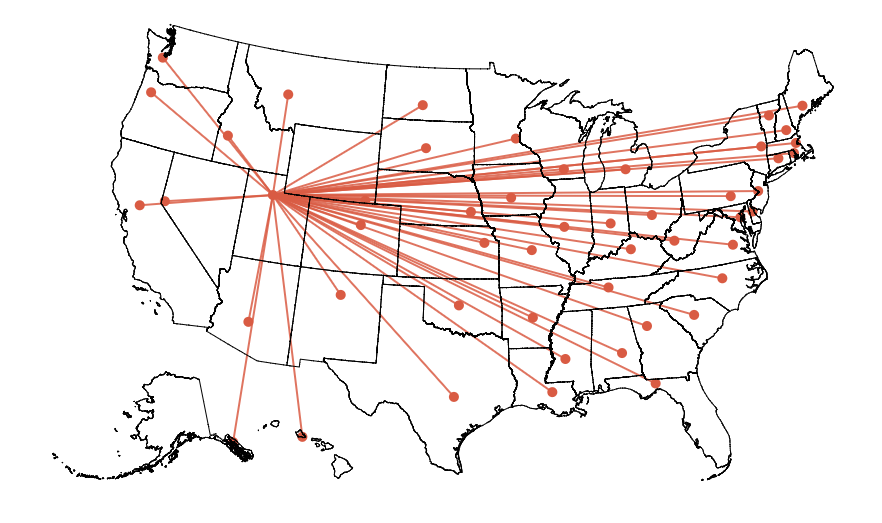
\includegraphics[width=12cm]{G:/CS6630/CS6630Project/proposal/source/airportConnection.PNG}
    \end{figure}
    \noindent The final appearance should be:\\
    $\diamond$ The initial image will show all the airports and highlight some important ones.\\
    $\diamond$ When any airport is selected, it will highlight all the airports which have flights from or to it.\\
    $\diamond$ The image will show the name, number of passengers, average delay of the selected airport and other useful related information.\\
    $\diamond$ The image will show flight lines connected to the selected airport.

    \subsection{statistical charts}
    \noindent $\diamond$ A bar chart to show annual change of the on-time performance of the current airport.\\
    $\diamond$ A bar chart to show monthly change of the on-time performance of the current airport.\\
    $\diamond$ A bar chart to show daily change of the on-time performance of the current airport.\\
    $\diamond$ A pie chart to show the distribution of the causes of flight delay.\\

\section{Optional Features}
    \subsection{Dynamic Effects}
    We will add some dynamic effects if possible. For each airline, we will draw the airplane with a small object. It will move back and forth along the airline according to the actual flight time. Then in the image we will be able to overview the running of the whole U.S. aviation system.
    \subsection{Mishandled-Baggage Rate, Denied Boarding Rate \& Consumer Complains}
    We will additionally summarize and analyze the mishandled Mishandled-Baggage Rate, Denied Boarding Rate and Consumer Complains for each airport and airline respectively.
    \subsection{Tips for the Airport}
    When each point on the map clicked it would show some kinds of tips for each airport. the information like the name of the airport and the enplanement for the airport and some data we calculated for this airport will also be displayed.
    \subsection{Airport Points Map}
    We will implement the map that is based on data instead of using US map : since we have a lot of airport data we may be able to construct the map with the data point (each data will have the location and we use scale to modify the location data for making our own map).
\section{Project Schedule}
\begin{table}[H]
\center
  \begin{tabular}{c|l}
  \hline
  Week & Assignment\\
  \hline
  1 & Cleanup and extract data\\
  2 & Build the frame and try to implement some basic features \\
  3 & Implement Must-have features \\
  4 & Implement Must-have features \\
  5 & Try to implement optional feature and review\\
  \hline
\end{tabular}
\end{table}



%\cite{2017delay}
%\cite{causes}
%\cite{Corrected}
%\cite{PTTF2015}
%\cite{AnnualReport2016}


\newpage
\renewcommand\refname{Reference}
\bibliographystyle{plain}
\bibliography{Reference}

\end{document}
